\section{Application of Trade-Off Model}

By calculating our two scores, ecological and economic, we can apply our impact score calculations to virtually any foreign species. For the purposes of our discussion, we chose two additional foreign plant species from the United States region: \textit{dandelions} in New York, \textit{garlic mustard plants} in Illinois, and  \textit{English ivy} plants in Washington. These foreign plants have practical social benefits and negatively affect their new environments \cite{columbiatribuneDandelionsFight, natureGarlicMustard, invasiveEnglishHedera}.

\subsection{Dandelion Plants}
\subsubsection{Ecological Impact Score}

As stated in the previous section, as part of determining the ecological impact score of dandelions, we need to examine their effect on native species. Thus, we chose the following ecologically related native species where dandelions reside in New York.

\begin{itemize}
    \item \textbf{Bombus impatiens} (Bumblebees) — native pollinators common to eastern North America that visit dandelion species \cite{nwfCommonEastern}.
    \item \textbf{Malacosoma americanum} (Moths) — feeds on the leaves of the common dandelion in New York. A consumer-plant relationship with dandelions \cite{butterfliesandmothsEasternTent}.
    \item \textbf{Cuscuta gronovii} (Scaldweed) — a climbing parasitic vine that extracts nutrients from attached-to plants \cite{minnesotawildflowersCuscutaGronovii}.
\end{itemize}

Below, we determined an interaction matrix for the Lotka-Volterra model based on the interactions of each species in row \(i\) to the species in column \(j\). For example, if species \(j\) was a natural predator of species \(i\), the value of \(\alpha_{ij}\) will be negative. If two species were mutualistic, we would expect that the element \(\alpha_{ij}\) would be positive, thus improving both population's growth rates. Note that generally, element \(\alpha_{ij} \neq \alpha_{ji}\) because the effect species \(i\) has on species \(j\) is generally opposite to the effect in the reverse order. Furthermore, the impact of the foreign species on native populations is found in the fourth row and fourth column of the matrix \(\alpha\).

Assuming a starting population of 100 plant units and a carrying capacity of 1000 plant units each, and a growth rate of 0.005 for bumblebees, as their populations mainly fluctuate by seasons, 0.06 for moths as their populations grow quickly, 0.01 for vines as their populations tend to stabilize, and 0.04 for dandelions as shown in the following logistic regression section \cite{nwfCommonEastern, butterfliesandmothsEasternTent, minnesotawildflowersCuscutaGronovii}. We solve the systems of differential equations (Equation~\ref{eq:lotkavolterra}) with the following approximated interaction matrix.

\begin{equation}
        \alpha_{\text{ dandelion}} = {\underbrace{\begin{bNiceMatrix}[first-row,first-col]
        &&&&& \\
    \text{Bumblebees} && 1 & 0.25 & -0.5 & 2 &\\
    \text{Moths} && 0.25 & 1 & 0.6 & 0 &\\
    \text{Vines} && -0.5 & -0.5 & 1 & 2 &\\
    \text{Dandelions} && 2 & 0.25 & -1 & 1 & \\
    \end{bNiceMatrix}}_{ \\ \text{3 native species, 1 foreign species}}}
\end{equation}

From graphing the population solutions to the system, we can visualize the population changes in Figure~\ref{fig:lotkavolterradandelion}. We find the change in populations over a single year to be \(\frac{1200}{100}\) for moths, \(\frac{250}{850}\) for vines, and \(\frac{550}{100}\) for bumblebees. So, we can calculate the native species impact score to be

\[\chi = \frac{1200}{100} + \frac{250}{850} + \frac{550}{100} = 17.794\]

\begin{figure}[h!]
\centering
    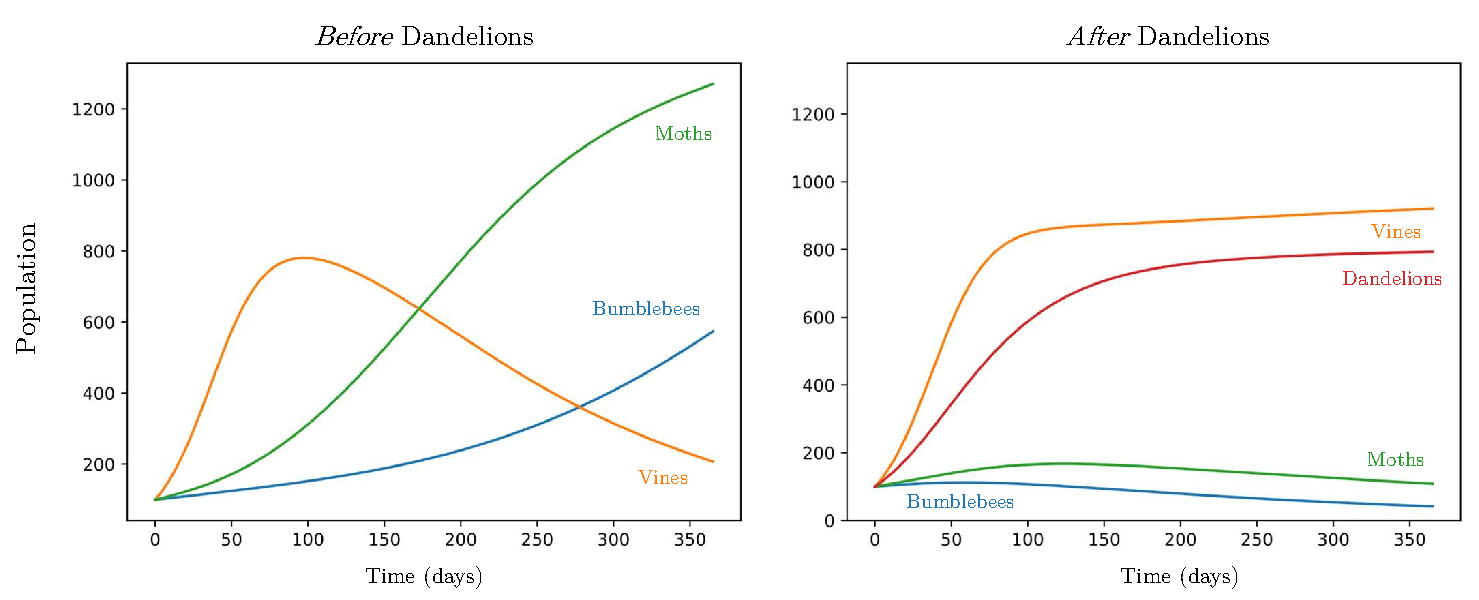
\includegraphics[scale=0.5]{figures/lotkavolterradandelions.pdf}
    \captionsetup{width=0.9\textwidth}
    \caption{\textbf{Impact of dandelion plants on native species populations}.}
    \label{fig:lotkavolterradandelion}
\end{figure}

Next, we calculate the spreadability index by performing logistic regression on dandelion population data from the previous model. We find that the carrying capacity of a region is approximately 900 dandelion plants (see Figure~\ref{fig:temperatepopulation}). Therefore, we calculate from logistic regression that the proportionality of growth is \(r = 0.04\); therefore, our spreadability score is \(100r = 4\).

Finally, we see that our total ecological impact score is \(4 + \chi = 4 + 17.794 = 21.794\) (Equation~\ref{eq:ecologicalimpact}).

\subsubsection{Economic Potential}

We constructed a small dandelion harvesting firm in New York to estimate economic profits. First, we can approximate the marginal cost of harvesting each dandelion to be around \(\$0.10\) per pound of dandelions \cite{farmshowGrowingDandelions, gardeningknowhowDandelionHarvest}. Next, we can also approximate the marginal revenue curve. Marginal revenue decreases for every five pounds of dandelions sold with maximum marginal revenue at around \(\$4.50\) per pound of dandelions \cite{farmfitlivingMakeMoney}.
So, we can model marginal revenue with a linear model with a slope of $-0.2$ and a y-intercept of $4.5$. By integration, we can calculate the total revenue and cost curves based on effort levels, shown in Figure~\ref{fig:dandelionprofits}. Therefore, we calculate dandelion profits (\(\pi_{\text{dandelions}}\)) be around \(\$47.86\).

\begin{figure}[h!]
\centering
    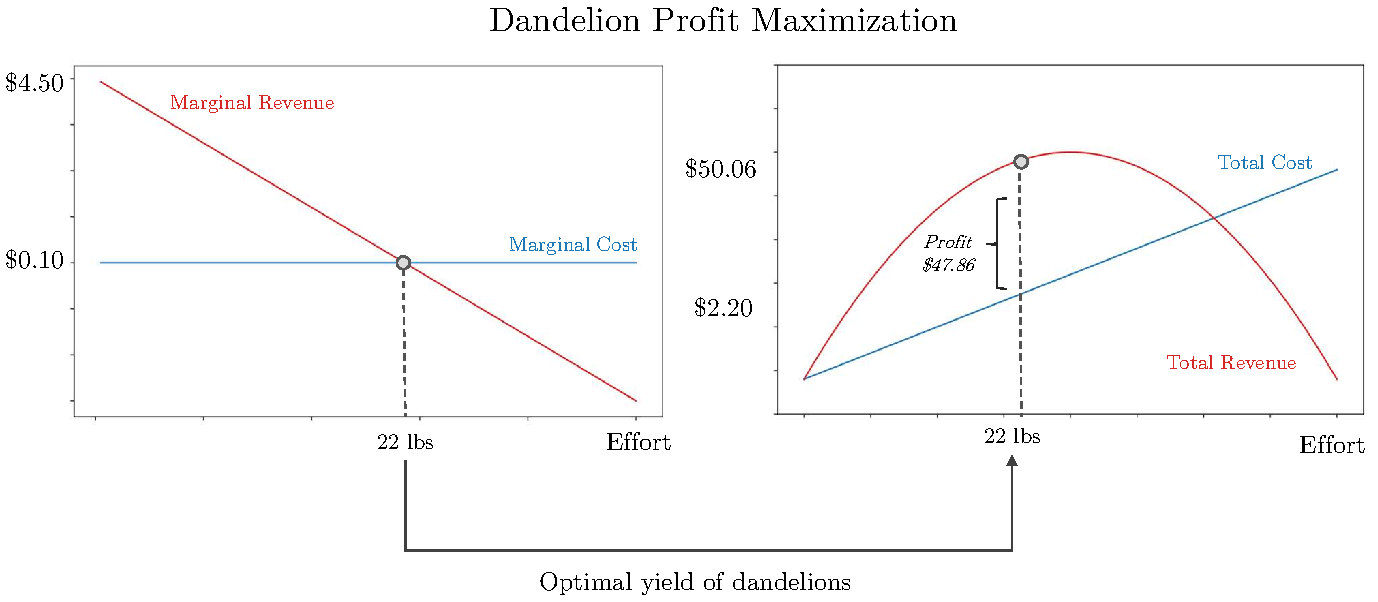
\includegraphics[scale=0.5]{figures/dandelionprofitmax.pdf}
    \captionsetup{width=0.9\textwidth}
    \caption{\textbf{Gordon-Schaefer model for dandelion profit yield.}}
    \label{fig:dandelionprofits}
\end{figure}

Additionally, we need to calculate the social welfare benefits and potential human risks. The typical population of an upstate New York town is approximately \(n = 60,000\), and the net external benefit for each individual is approximately \(\$0.002\) as dandelions are a rarely used medicinal plant and scarcely found soil loosener \cite{healthlineDandelionHealth}. Lastly, New York's Gini coefficient is 0.52 \cite{statistaBetweenRich}. Incorporating these aspects, the social welfare output is: \[W = (1- 0.52) \sum_{i = 1}^{60000} 0.002 = \$57.60\].

Finally, we need to find the human health risk by calculating the amount of harm a dandelion has on its surrounding human population. Because dandelions do not generally seriously harm humans, we assign the potential human risk to be \(R = 0\).

With the three components of the economic \textit{potential} score, we can calculate the total economic \textit{benefit} score to be 

\[\text{Total Economic Benefit } = \pi + W - R = 47.86 + 57.60 - 0 = \$105.46\]

So, our final invasive species impact score is

\[\text{Impact Score} = (\text{Ecological Score, Economic Score}) = (21.794, \$105.46)\]

\subsection{Garlic Mustard Plants}

\subsubsection{Ecological Impact Score}

Next, to determine the ecological impact score of garlic mustard plants, we chose the following ecologically related native species where garlic mustard plants reside in Illinois.

\begin{itemize}
    \item \textbf{White trillium} (Wildflower) — a native wildflower that grows in woodlands and is often threatened by garlic mustard invasion \cite{usdaGreatWhite}.
    \item \textbf{Plethodon cinerus} (Salamander) — an amphibian that lives under leaves and feeds on insects \cite{amphibiawebAmphibiaWebPlethodon}.
    \item \textbf{Hylocichla mustelina} (Wood thush) — a songbird that nests in forests where garlic mustard invasion reduces vegetation for nesting cover \cite{allaboutbirdsWoodThrush}.
\end{itemize}

Below, we again determine an interaction matrix for the Lotka-Volterra model. Note that we again assume that the starting population of each species is 100 units with a carrying capacity of 1000 plant units each. We also assume a growth rate of 0.06 for wildflowers, as their populations mainly fluctuate by seasons, 0.03 for salamanders as their populations do not grow as quickly, 0.01 for songbirds as their populations tend to stabilize, and 0.1 for garlic mustard plants as their populations tend to proliferate. We finally solve the systems of differential equations shown in Equation~\ref{eq:lotkavolterra} with the following interaction matrix (Equation~\ref{eq:garlicmustardinteraction}).

\begin{equation}
        \alpha_{\text{ garlic mustard}} = {\underbrace{\begin{bNiceMatrix}[first-row,first-col]
        &&&&& \\
    \text{Wildflower} && 1 & 0.75 & 1.5 & -1 &\\
    \text{Salamanders} && 0.35 & 1 & 0.65 & -1 &\\
    \text{Songbirds} && 0.5 & 0.5 & 1 & -1 &\\
    \text{Garlic mustard} && 0.25 & 0.25 & 0.15 & 1 &\\
    \end{bNiceMatrix}}_{ \\ \text{3 native species, 1 foreign species}}}
    \label{eq:garlicmustardinteraction}
\end{equation}

In the fourth column of \(\alpha_{\text{ garlic mustard}}\), we assigned a value of -1 to each element since garlic mustard plants harm all three native species populations.  

By graphing the population solutions to the system, we can see the population changes in Figure~\ref{fig:lotkavolterragarlicmustard}. We find the ratio of change of populations over a single year to be \(\frac{150}{100}\) for wildflowers, \(\frac{800}{450}\) for salamanders, and \(\frac{400}{200}\) for songbirds. So, we can calculate the native species impact score to be

\[\chi = \frac{150}{100} + \frac{800}{450} + \frac{400}{200} = 5.278\]

\begin{figure}[h!]
\centering
    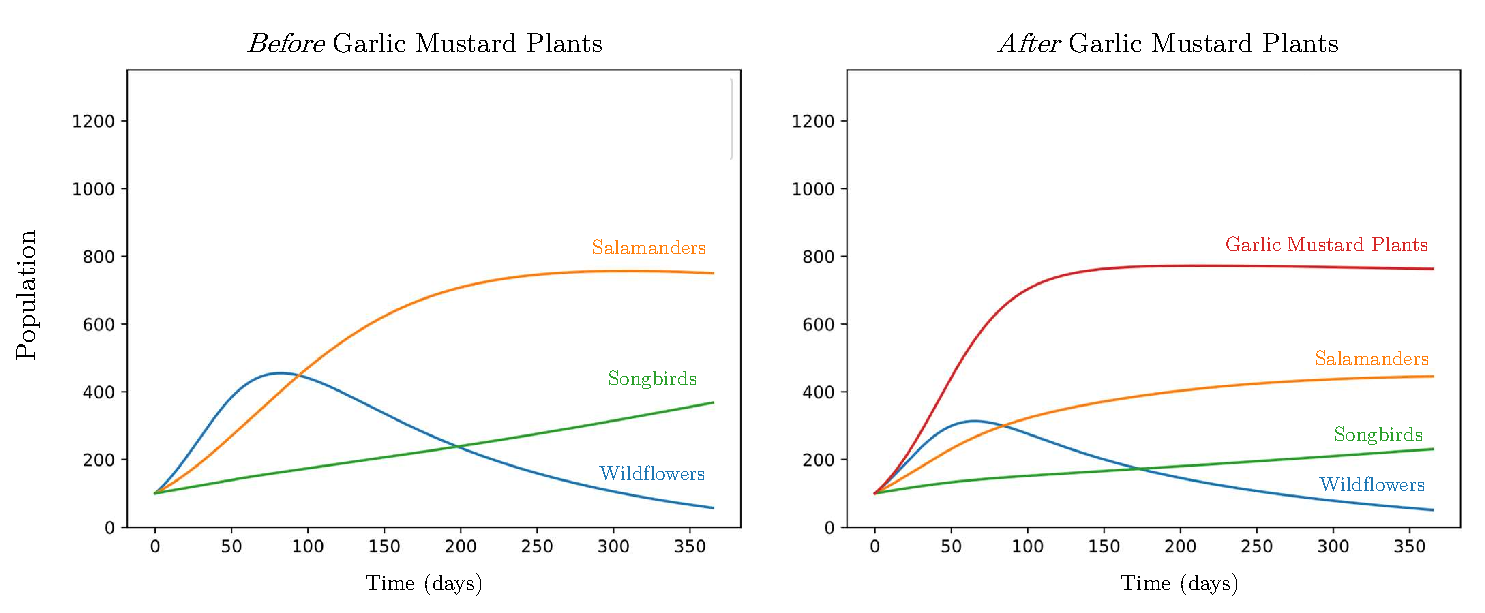
\includegraphics[scale=0.5]{figures/lotkavolterragarlicmustard.pdf}
    \captionsetup{width=0.9\textwidth}
    \caption{\textbf{Impact of garlic mustard plants on native species populations}.}
    \label{fig:lotkavolterragarlicmustard}
\end{figure}

To calculate the spreadability index, we can start from an accepted fact that garlic mustard populations can double in a year in most growing conditions \cite{fmrInvasiveSpecies}. Therefore, by performing logistic regression with the $x$-axis being days and the \(y\)-axis as population, we observe that the \(r\) value is around 0.05. So, our spreadability index can be calculated as \(100r = 5\). Thus, by Equation~\ref{eq:ecologicalimpact}, our ecological impact score is \(5 + \chi = 5 + 5.278 = 10.278\).

\subsubsection{Economic Potential}

As harvesting efforts for garlic mustard plants are minimal (we could not find any garlic mustard plant products via an online search), we conclude there is no possibility of a garlic mustard harvesting firm. This means that there is \textit{no potential economic profit} (\(\pi = 0\)).

Next, we calculate a garlic mustard plants' social welfare benefits. The population of a typical town in Illinois is approximately \(n = 50,000\), and the net external benefit for each individual person is similar to dandelions at approximately \(\$0.001\) as garlic mustard plants are a rarely used medicinal herb \cite{fmrInvasiveSpecies}. Furthermore, the Gini coefficient for Illinois is 0.48 \cite{247wallstIncomeInequality}, hence, the social welfare output is \[W = (1- 0.48) \sum_{i = 1}^{50000} 0.001 = \$26.00\].

Lastly, we determine the human health risk by calculating the amount of harm garlic mustard plants have on its surrounding human population. Because dandelions do not generally seriously harm humans, we assign the potential human risk to be \(R = 0\).
\cite{fmrInvasiveSpecies}.

With the three components of the economic potential score, we can calculate the score to be 

\[\text{Total Economic Benefit } = \pi + W - R = 0 + 26.00 - 0 = \$26.00\]

So, our final invasive species impact score for garlic mustard plants is

\[\text{Impact Score} = (\text{Ecological Score, Economic Score}) = (5.278, \$26.00)\]

\subsection{English Ivy Plants}

\subsubsection{Ecological Impact Score}

To determine the ecological impact score of English ivy plants, we examine the top 3 most closely related native species where English ivy plants reside in Washington:

\begin{itemize}
    \item \textbf{Kinnikinnick} (Shrub) — an evergreen shrub that grows in most conditions and attracts a variety of native pollinators and birds \cite{wnpsPlantProfile}.
    \item \textbf{Asarum caudatum} (Wild ginger) — a low-lying groundcover plant with edible leaves \cite{portlandnurseryAsarumCaudatum}.
    \item \textbf{Mahonia aquifolium} (Oregon grape) — another evergreen plant that produces berries and can grow in most temperate conditions in Washington \cite{oregonstateMahoniaAquifolium}.
\end{itemize}

For the last time, we determine an interaction matrix for the Lotka-Volterra model. We again assume that each species' starting population is 100 units with a carrying capacity of 1000 plant units each. We assume a growth rate of 0.02 for shrubs, as their populations mainly fluctuate by season, 0.04 for wild gingers as their populations grow rapidly across forest floors, 0.01 for Oregon grapes as their populations tend to stabilize, and 0.4 for English ivy plants as their populations tend to multiply. We solve the new Lotka-Volterra system with the following interaction matrix.

\begin{equation}
        \alpha_{\text{ english ivy}} = {\underbrace{\begin{bNiceMatrix}[first-row,first-col]
        &&&&& \\
    \text{Shrubs} && 1 & 0 & -0.5 & -0.25 &\\
    \text{Wild ginger} && 0 & 1 & 0 & -1 &\\
    \text{Oregon grape} && -0.5 & 0 & 1 & -1 &\\
    \text{English ivy} && 0.25 & -1 & 0.15 & 1 &\\
    \end{bNiceMatrix}}_{ \\ \text{3 native species, 1 foreign species}}}
\end{equation}

In \(\alpha_{\text{ english ivy}}\), several elements are set to zero because they live in independent habitats, meaning they rarely compete for the same natural resources. However, English ivy plants compete vigorously with wild ginger, so the respective elements are \(-1\) \cite{portlandnurseryAsarumCaudatum}.

\begin{figure}[h!]
\centering
    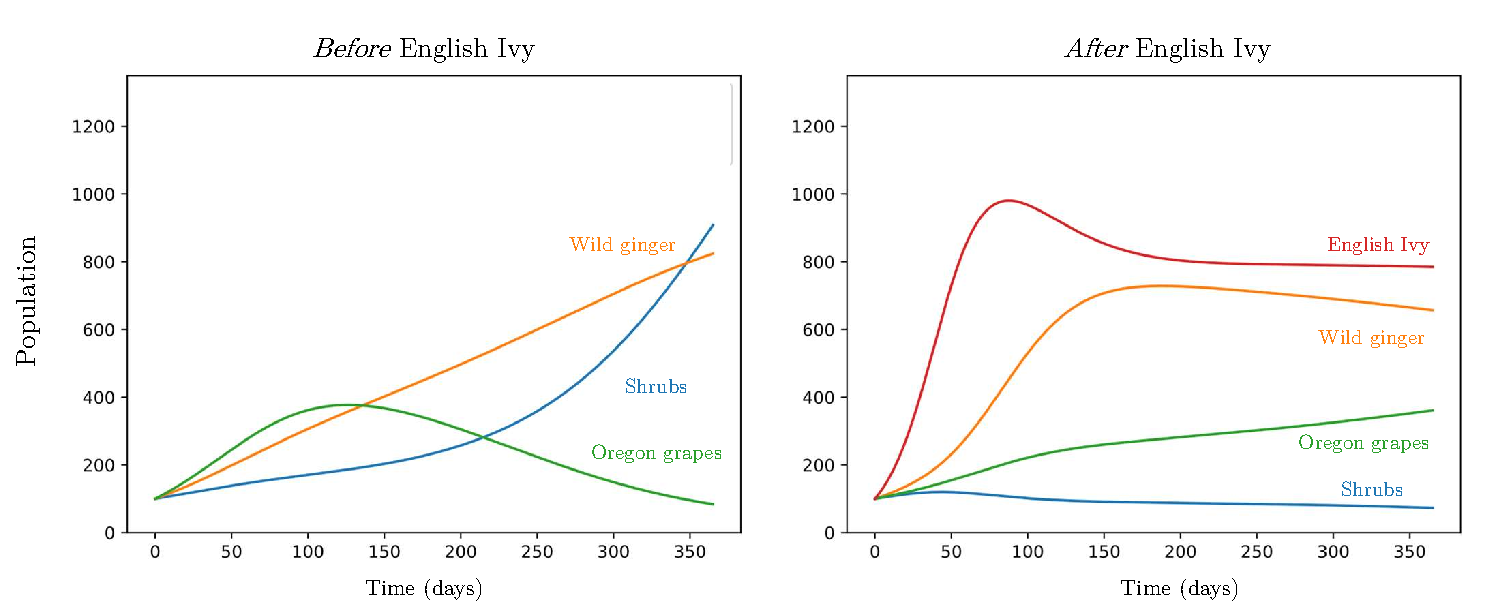
\includegraphics[scale=0.5]{figures/lotkavolterraenglishivy.pdf}
    \captionsetup{width=0.9\textwidth}
    \caption{\textbf{English ivy impact on native species populations.}}
    \label{fig:lotkavolterraenglishivy}
\end{figure}

By graphing the population solutions to the system, we can see the population changes in Figure~\ref{fig:lotkavolterraenglishivy}. We find the change of populations over a single year to be \(\frac{900}{90}\) for shrubs, \(\frac{800}{600}\) for wild ginger, and \(\frac{100}{300}\) for Oregon grapes. So, we calculate the native species impact score to be

\[\chi = \frac{900}{90} + \frac{800}{600} + \frac{100}{300} = 11.667\]

Next, we determine the spreadability index. We can start with an accepted fact that English ivy populations can double in around one and a half years in most growing conditions, even in the shade \cite{usdaHederaHelix}! Therefore, by performing logistic regression with the x-axis being days and the y-axis as population, we find that the \(r\) value is around 0.035. So, our spreadability index is calculated as \(100r = 3.5\). Therefore, by Equation~\ref{eq:ecologicalimpact}, our ecological impact score is \(3.5 + \chi = 3.5 + 11.667 = 15.167\).

\subsubsection{Economic Potential}
We assume that there exists some small landscaping firm that harvests and grows English ivy plants in a typical town in Washington, as many landscaping designers use English ivy to decorate their clients' backyards \cite{psuEnglishLandscape}. By analyzing the microeconomic model of this firm, we will be able to calculate our economic profits.

First, we estimate the expected marginal cost and revenue of harvesting and growing each pound of English ivy based on the Gordon-Schaefer model. We estimate that the constant marginal cost of harvesting each pound of English ivy is around \(\$15.00\), as it takes around an hour of manual labor to safely harvest English ivy \cite{bhgCaringEasytoGrow}. 

To model marginal revenue, we surveyed online shopping sources to estimate the revenue per pound of English ivy. Based on several pricing estimates \cite{gardengoodsdirectEnglish}, we conclude that the maximum pricing for a pound of English ivy would fall around \(\$100.00\) and decrease with slope \(-0.5\) per pound increased of English ivy. After applying the Profit Maximization Law, analyzing this firm with the Gordon-Schaefer model, and finding the intersection of the MR and MC curve, an optimal English ivy yield would be around 170 lbs for \(\$57.75\) per pound. 

To calculate economic profits (\(\pi\)), we subtract total costs (\(\$15.00 \cdot 170\)) from total revenue (\(\$57.75 \cdot 170\)), which leads us to conclude that \(\pi = \$7225.00\).

As for measuring social welfare, English ivy has no benefits to humans other than as a landscaping plant, which is already an integral part of economic profits. Lastly, for the human risk factor, English ivy is inedible and contains toxic sap (yuck!). However, English ivy plants rarely harm humans. Therefore, we deduce that social welfare \(W = 0\) and human risk \(R = 0\). So, our total economic potential can be calculated as 

\[\text{Total Economic Benefit } = \pi + W - R = \$7225.00\]

So, our final invasive species impact factor for English ivy plants in Washington is

\[\text{Impact Score} = (\text{Ecological Score, Economic Score}) = (15.167, \$7225.00)\]

\subsection{Score Comparison}

To analyze the differences in each score and the "classification" of each foreign species, we look at the trade-offs between ecological and economic scores in our definition of an impact factor.

\begin{table}[h]
\renewcommand{\arraystretch}{1.3}
%p{0.8\linewidth
    \begin{tabularx}{\textwidth}{p{0.18\textwidth}llX}
    \toprule
    \textbf{Foreign Species}  & \textbf{Ecological} & \textbf{Economic} & \textbf{Analysis} \\ \midrule
    \raggedright Dandelions & 21.794 & \(\$105.46\) & As dandelions have a high ecological impact primarily due to the loss of native populations with a low return in economic potential, we conclude that dandelions are indeed \textit{invasive species}. \\
    \rowcolor{gray!15}
    \raggedright Garlic mustard & 5.278  & \(\$26.00\) & Since garlic mustard plants have a slight ecological impact and have little to no return on economic potential, we label garlic mustard plants as \textit{invasive species.}\\
    \raggedright English ivy & 15.167 & \(\$7225.00\) & As English ivy plants have a high impact on the environment yet also have a large return on economic potential, we conclude that English ivy plants \textit{are not invasive}.\\
    \bottomrule
    \end{tabularx}
\end{table}